\documentclass{article}
\usepackage[margin=1in]{geometry}
\usepackage{tikz}
\usetikzlibrary{calc}

\title{Force}
\author{Andrew Carter}

\begin{document}
\maketitle

\section{Potential}
Force particles are emitted in random directions from a matter particle.
The force particle then deposit potential on nearby matter particles in some manner.
The overall force on a particle is based on a function of the potentials of nearby particles.

\begin{figure}[h!]
\centering
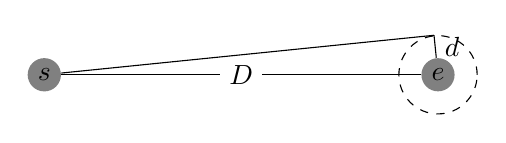
\begin{tikzpicture}
[place/.style={circle,fill=gray,inner sep=2pt},
 bubble/.style={circle,draw,dashed,inner sep=10pt}]

\node (s) at (0,0) [place] {$s$};
\node (e) at (5,0) [place] {$e$};
\node (r) at (e.center) [bubble]{};

\draw (e) -- (s) node [midway,fill=white]{$D$};
\draw (e) -- (tangent cs:node=r,point={(s)},solution=2) node [midway,right]{$d$};
\draw (s) -- (tangent cs:node=r,point={(s)},solution=2);
\end{tikzpicture}
\label{fig:potential}
\caption{Diagram for the potential on a particle.}
\end{figure}

In general, consider the various ways to calculate the potential created be the source particle $s$ and deposited on $e$ some distance $D$ away as shown in Figure \ref{fig:potential}.
Furthermore, $e$ only cares about force particles in the local vicinity $d$.
Finally, $s$ releases particles at some rate $k_r$, each having some constant $k_p$ associated with them, and the potential on $e$ decays at some rate $k_d$.

\subsection{Equilibrium}
A potential is in equilibrium with respect to another particle when the rate at which potential is deposited on the particle is equal to the rate at which potential decays on the particle.
If potential increases at a rate of $dP$ due to deposits from force particles, then because potential degrades at a rate of $k_d$, the potential is in equilibrium when $dP - k_d P = 0$.

We can let $dP = \sum_i dP_i$ where $dP_i$ is the rate of increase from a particular particle, and $P_i$ is the total accumulation of potential due to that particle, then
$$\sum_i dP_i - k_d\sum_i P_i = 0,$$
we can set each of the terms equal so the potential is in equilibrium when $dP_i = k_d P_i$ for all $i$, or
\begin{equation}
P_{i_{eq}} = \frac{1}{k_d} dP_i
\label{eq:equilibrium}
\end{equation}

\section{Vicinity Potential}
Whenever a force particle is in the vicinity of a matter particle it deposits potential inversely proportional to the distance the particle has traveled.
For continuous deposits one a two dimensional system with $d < D$, the rate that potential is deposited is equal to 
$$
\frac{k_r}{2\pi}
\int_{-\sin^{-1}(d/D)}^{\sin^{-1}(d/D)}
\int_{D \cos(\theta) - D\sqrt{(d/D)^2 - \sin^2(\theta)}}^{D \cos(\theta) + D\sqrt{(d/D)^2 - \sin^2(\theta)}}
\frac{k_p}{r} r dr d\theta
$$
This simplifies to
\begin{equation}
\frac{k_rk_pD}{\pi}
\int_{-\sin^{-1}(d/D)}^{\sin^{-1}(d/D)}
\sqrt{(d/D)^2 - \sin^2(\theta)}d\theta,
\label{eq:vp near int}
\end{equation}
which integrates to some elliptic curve, 
\begin{equation}
\frac{2k_rk_pd}{\pi} E\left(\frac{d}{D},\frac{D}{d}^2\right).
\label{eq:vp near}
\end{equation}

However for $D >> d$ we can simplify $\sin(d/D) \approx d/D$ which turns $\ref{eq:vp near int}$ into
$$
\frac{k_rk_pD}{\pi}
\int_{-d/D}^{d/D}
\sqrt{(d/D)^2 - \theta}d\theta,
$$
which integrates to
\begin{equation}
\frac{k_rk_pd^2}{2} \frac{1}{D}.
\label{eq:vp far}
\end{equation}

\section{Force}
The force between any two nearby particles is equal to the difference in potential between the two particles divided between the distance between the particles.

\begin{figure}[h!]
\centering
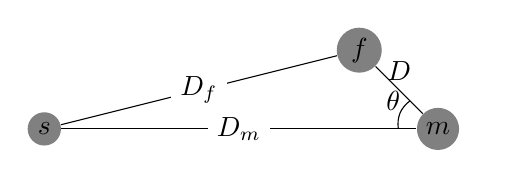
\begin{tikzpicture}
[place/.style={circle,fill=gray,inner sep=2pt},
 bubble/.style={circle,inner sep=10pt}]
 
\node (s) at (0,0) [place] {$s$};
\node (m) at (5,0) [place] {$m$};
\node (f) at (4,1) [place] {$f$};

\node (arc) at (5,0) [bubble] {};



\draw (s) -- (m) node (sm) [midway,fill=white]{$D_m$};
\draw (s) -- (f) node (sf) [midway,fill=white]{$D_f$};
\draw (m) -- (f) node (mf) [midway,above]{$D$};

\draw[bend left] (intersection 1 of arc and m--s) to (intersection 1 of arc and m--f) node [left] {$\theta$};
\end{tikzpicture}
\label{fig:force}
\caption{Diagram for the force between two particles due to a third particle.}
\end{figure}

Consider the relative force from $f$ on a matter particle $m$ due to the force particles from $s$.
Let $D_m$ be the distance from $s$ to $m$, $\theta$ be the angle $s, m, f$ and $D$ be the distance between $m$ and $f$ as shown in Figure \ref{fig:force}.

Consider the case when the equilibrium potential on $m$ and $f$ due to $s$ be inversely proportional to the distance between them.
Therefore the equilibrium potential on $m$ due to $s$, $P_m = k/D_m$ and similarly $P_f = k/D_f$.
The overall force
$$F = \frac{k}{D}\left(\frac{1}{D_m} - \frac{1}{D_f}\right),$$
We know that $D_f^2 = D^2 + D_m^2 - 2 D D_m \cos(\theta)$, therefore
$$F = \frac{k}{D}\left(\frac{1}{D_m} - \frac{1}{\sqrt{D^2 + D_m^2 - 2 D D_m \cos(\theta)}}\right),$$
$$F = \frac{k}{D^2}
\frac{1 + \frac{D_m}{D}^2 - 2 \frac{D_m}{D} \cos(\theta) - \frac{D_m}{D} \sqrt{1 + \frac{D_m}{D}^2 - 2 \frac{D_m}{D}\cos(\theta)}}
{\frac{D_m}{D}\left(1 + \frac{D_m}{D}^2 - 2 \frac{D_m}{D} \cos(\theta)\right)},
$$
If $D << D_m$ then,
$$1 + \frac{D_m}{D}^2 - 2 \frac{D_m}{D}\cos(\theta) \approx 1,$$
$$\sqrt{1 + \frac{D_m}{D}^2 - 2 \frac{D_m}{D}\cos(\theta)} \approx 1 + \frac{1}{2}\frac{D_m}{D}^2 - \frac{D_m}{D}\cos(\theta),$$
resulting in
\begin{equation}
F = k\frac{\left(\frac{D_m}{D} - \cos\left(\theta\right)\right)}{2D^2}
\label{eq:force approx}
\end{equation}

\section{Application to Our Universe}

Note that as $\theta \to \pm \frac{\pi}{2}$ that $F \to 0$ in Equation \ref{eq:force approx}, and otherwise if $\cos\left(\theta\right)$ is large then
$$F \approx -\frac{k}{2}\cos\left(\theta\right)\frac{1}{D^2},$$
in either case $F$ approximates the force component due to the original particle.

In order for this method to work, empty space needs to be filled with fake particles.
A matter particle cannot directly exert force on another matter particle, but must create potential on another particle instead.
Additionally the distances between particles must be small for this approximation to work.

The force may also be proportional inversely to the total potential on the object.
Since gravity is only additive, then there may be an excess amount of gravitational potential relative to electric potential.
The electric potential may be dominated by the potential radiating from the source (which in the continuous approximation is infinite), however in a discrete model it is merely very large.
Since all electric particles have the same amount of charge (or are very close and have a charge that adds up to $1$) there would be no way to tell.
Similarly the universe is saturated with a certain level of gravitational potential, which is orders of magnitude greater than the charge on a single particle, then all particles will have approximately the same base potential.




\end{document}